\documentclass{beamer}
\usepackage{ctex, hyperref}
\usepackage[T1]{fontenc}

% other packages
\usepackage{latexsym,amsmath,xcolor,multicol,booktabs,calligra}
\usepackage{graphicx,pstricks,listings,stackengine}

\author{Elain Bai, Yanhui Li, Weiqi Zhang}
\title{JLU TAG}
\subtitle{}
\institute{Jilin University}
\date{2023.11.15}
\usepackage{JilinUniv}

% defs
\def\cmd#1{\texttt{\color{red}\footnotesize $\backslash$#1}}
\def\env#1{\texttt{\color{blue}\footnotesize #1}}
\definecolor{deepblue}{rgb}{0,0,0.5}
\definecolor{deepred}{rgb}{0.6,0,0}
\definecolor{deepgreen}{rgb}{0,0.5,0}
\definecolor{halfgray}{gray}{0.55}

\lstset{
    basicstyle=\ttfamily\small,
    keywordstyle=\bfseries\color{deepblue},
    emphstyle=\ttfamily\color{deepred},    % Custom highlighting style
    stringstyle=\color{deepgreen},
    numbers=left,
    numberstyle=\small\color{halfgray},
    rulesepcolor=\color{red!20!green!20!blue!20},
    frame=shadowbox,
}


\begin{document}

\kaishu
\begin{frame}
    \titlepage
    \begin{figure}[htpb]
        \begin{center}
            
\includegraphics[width=0.15\linewidth]{pic/Jilin_University_Logo.eps}
        \end{center}
    \end{figure}
\end{frame}

\begin{frame}
\tableofcontents[sectionstyle=show,subsectionstyle=show/shaded/hide,subsubsectionstyle=show/shaded/hide]
\end{frame}

\section{Project description}

\begin{frame}{Contributors}
    \begin{itemize}
        \item Data Scientist: Elain Bai
        \item Domain Expert: Elain Bai, Yanhui Li
        \item Knowledge Engineer: Elain Bai, Weiqi Zhang
        \item Project Manager: Elain Bai
        \item Teacher: Rui Zhang
    \end{itemize}
\end{frame}

\begin{frame}{Pixiv}
    \begin{figure}[l]
        \centering
        
\includegraphics[height=.08\textheight]{pic/pixiv.png}
    \end{figure}
\end{frame}

\begin{frame}{Project description}
    \begin{itemize}
        \item This project aims to use knowledge graph technology to organize the tags of illustrations on websites such as Pixiv and Lofter to provide a better user experience. We build a knowledge graph to provide a structured representation of information about illustration works, characters, etc., and provide basic data for classification.
        \item Usage Scenarios: 
        \par Users can browse the illustrations on the above-mentioned websites more conveniently and find the content they are interested in through searches combined with the knowledge graph.
    \end{itemize}
\end{frame}

\section{Data resources}

\begin{frame}{Data resources}
    \begin{itemize}
        \item First of all, the largest illustration website in the world is Pixiv. We can crawl the illustration tag data from this website. We then crawled data about characters and titles from encyclopedia sites like Moegirl and Bangumi.
        \item We first determine the crawling target, then choose the crawler tool to crawl, and finally store the crawled data in JSON form.
    \end{itemize}
\end{frame}

\section{Knowledge Graph}

\begin{frame}{}
    \begin{figure}[l]
        \centering
        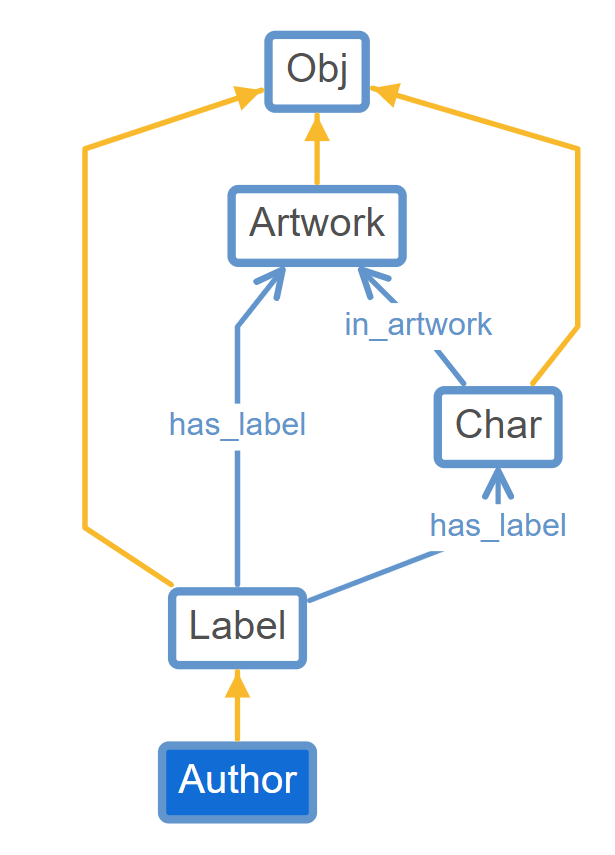
\includegraphics[height=.8\textheight]{pic/protege.png}
    \end{figure}
\end{frame}

\begin{frame}{KG}
    \begin{figure}[l]
        \centering
        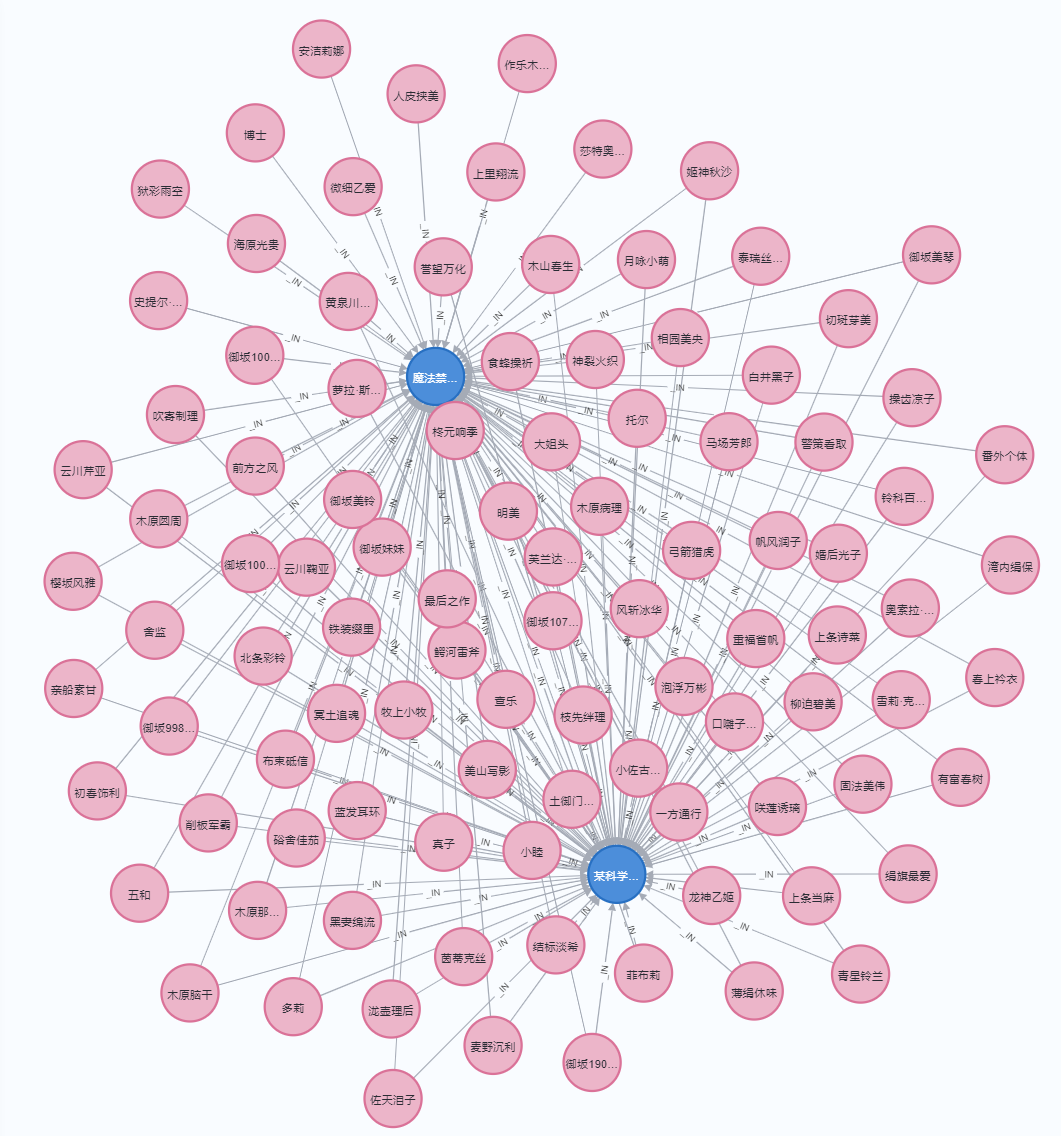
\includegraphics[height=.8\textheight]{pic/2.png}
    \end{figure}
\end{frame}

\begin{frame}{}
    \begin{figure}[l]
        \centering
        
\includegraphics[height=.5\textheight]{pic/11.png}
    \end{figure}
\end{frame}

\begin{frame}{}
    \begin{figure}[l]
        \centering
        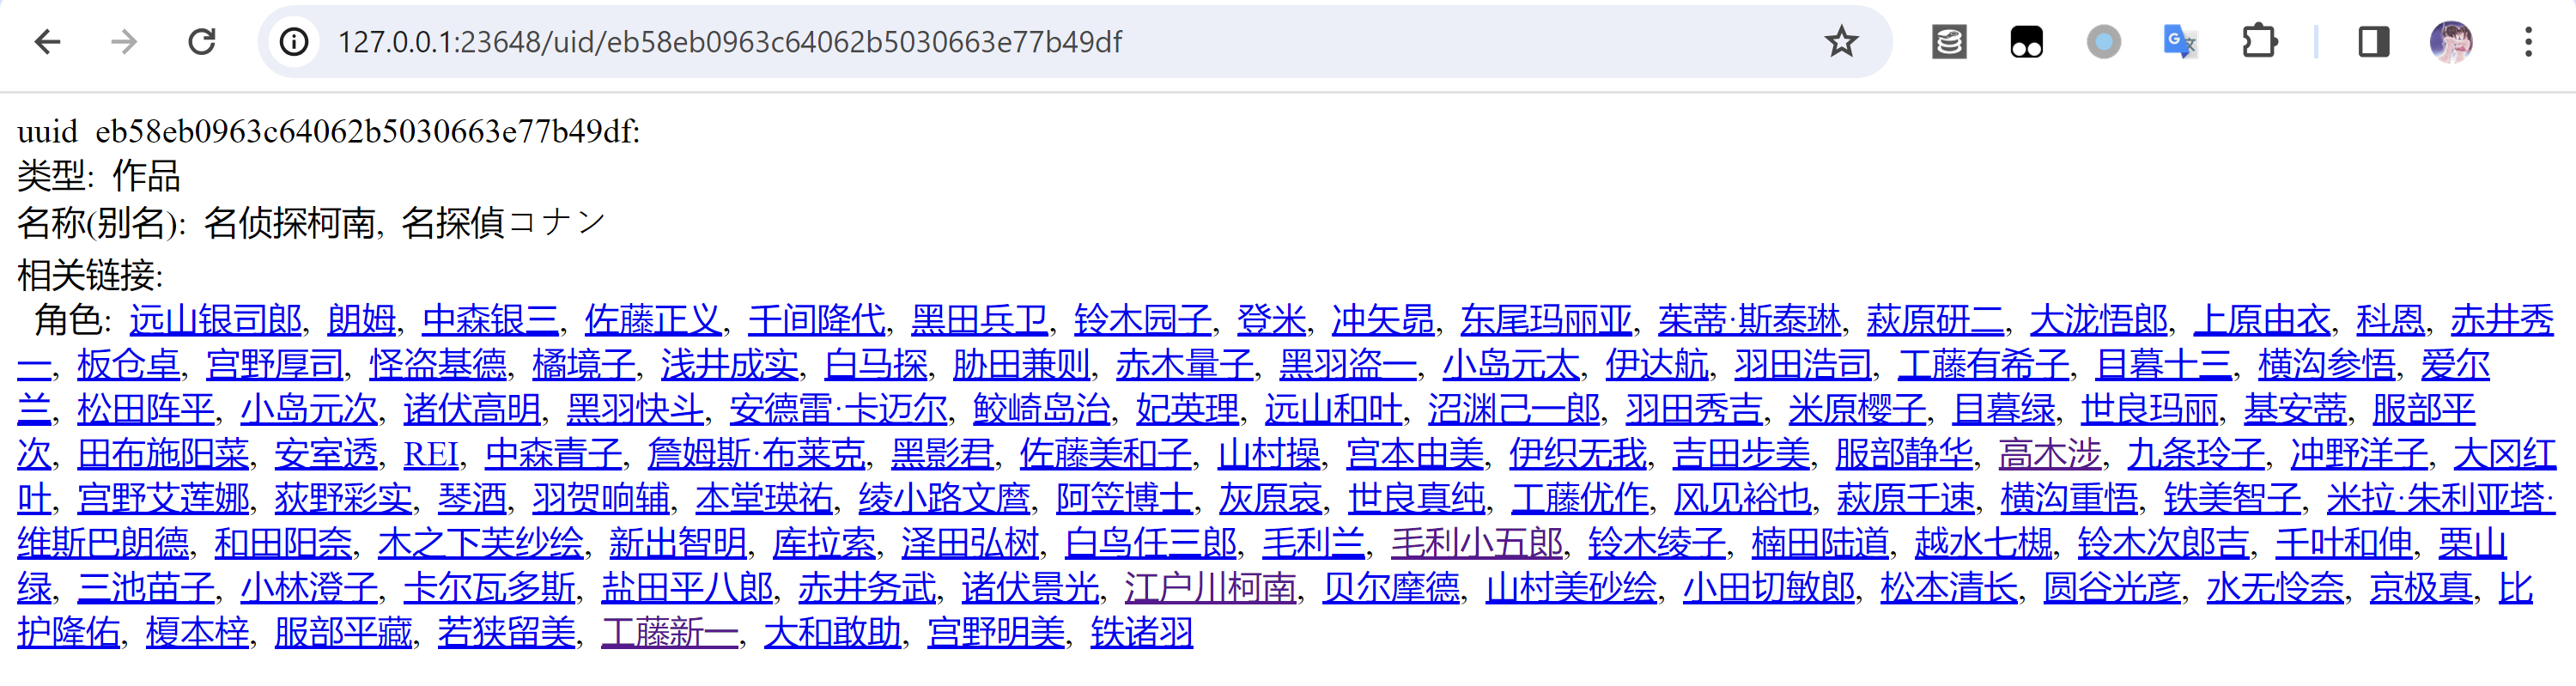
\includegraphics[height=.3\textheight]{pic/13.png}
    \end{figure}
\end{frame}

\begin{frame}{}
    \begin{figure}[l]
        \centering
        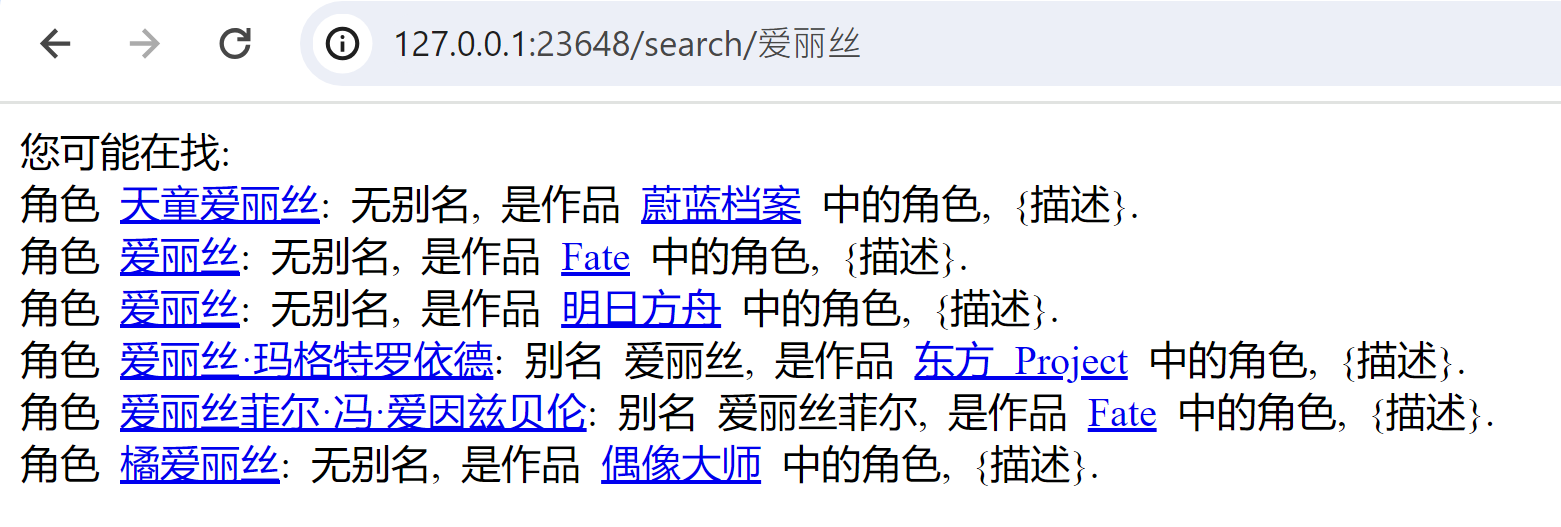
\includegraphics[height=.5\textheight]{pic/12.png}
    \end{figure}
\end{frame}


\section{Problems and Solutions}

\begin{frame}{Anti-crawling}
    \begin{figure}[l]
        \centering
        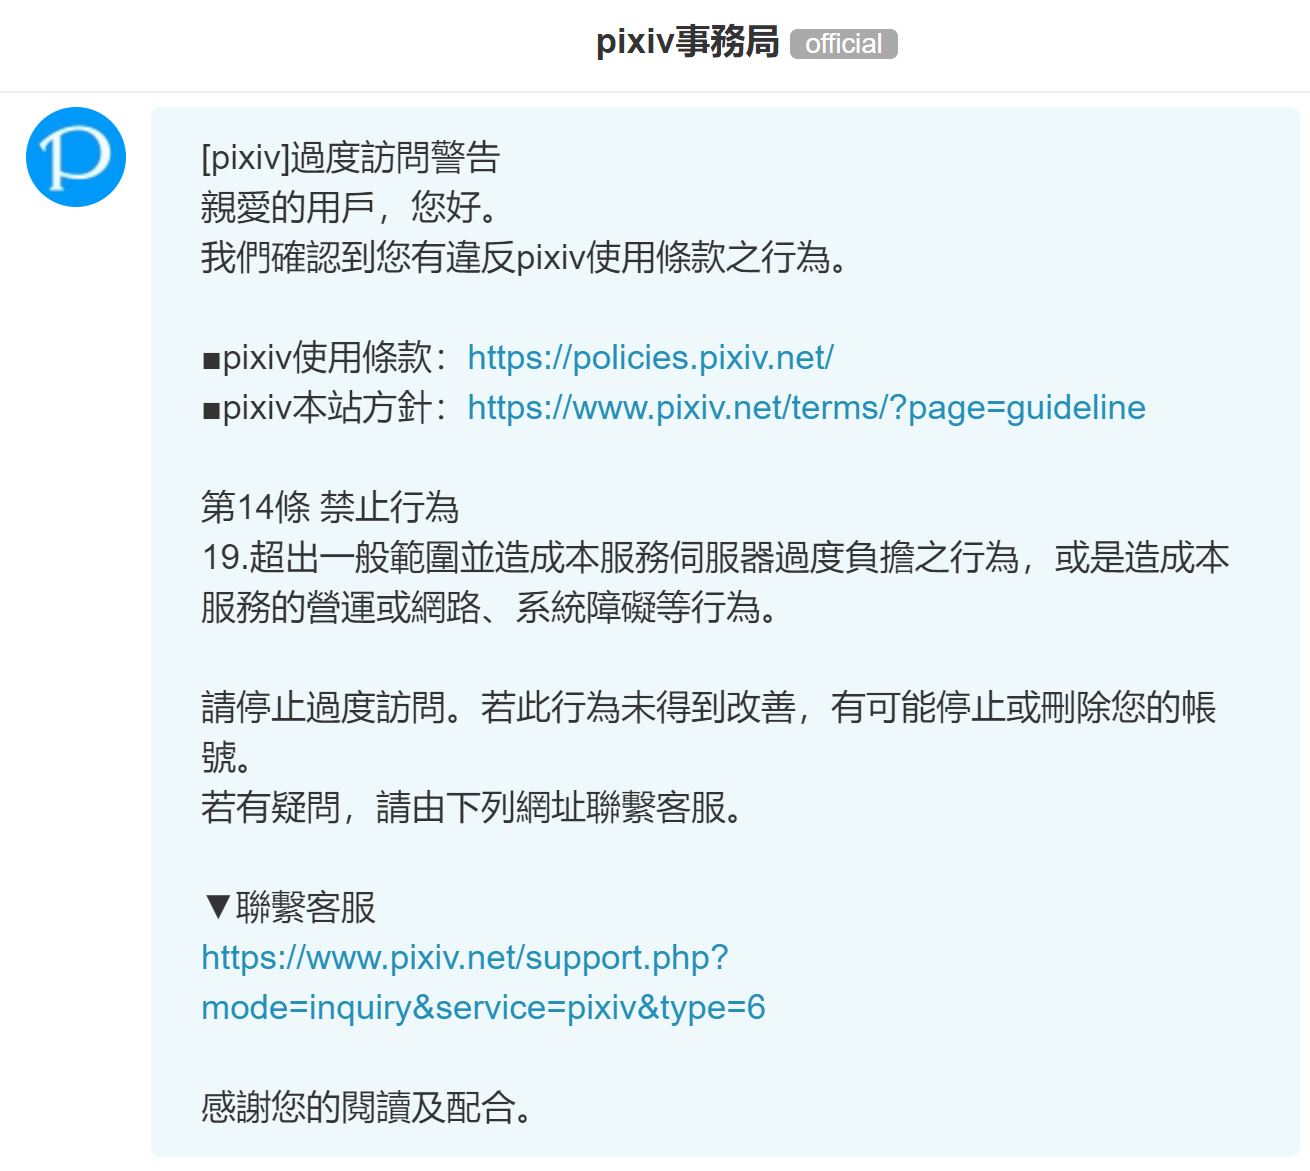
\includegraphics[height=.8\textheight]{pic/anti.png}
    \end{figure}
\end{frame}

\begin{frame}{Huge amount of data}
    \begin{itemize}
        \item The amount of data on the Pixiv, Moegirl and Bangumi is very large, and processing large-scale data may affect the efficiency and speed of the project.
    \end{itemize}
\end{frame}

\begin{frame}{System limitations}
    \begin{figure}[l]
        \centering
        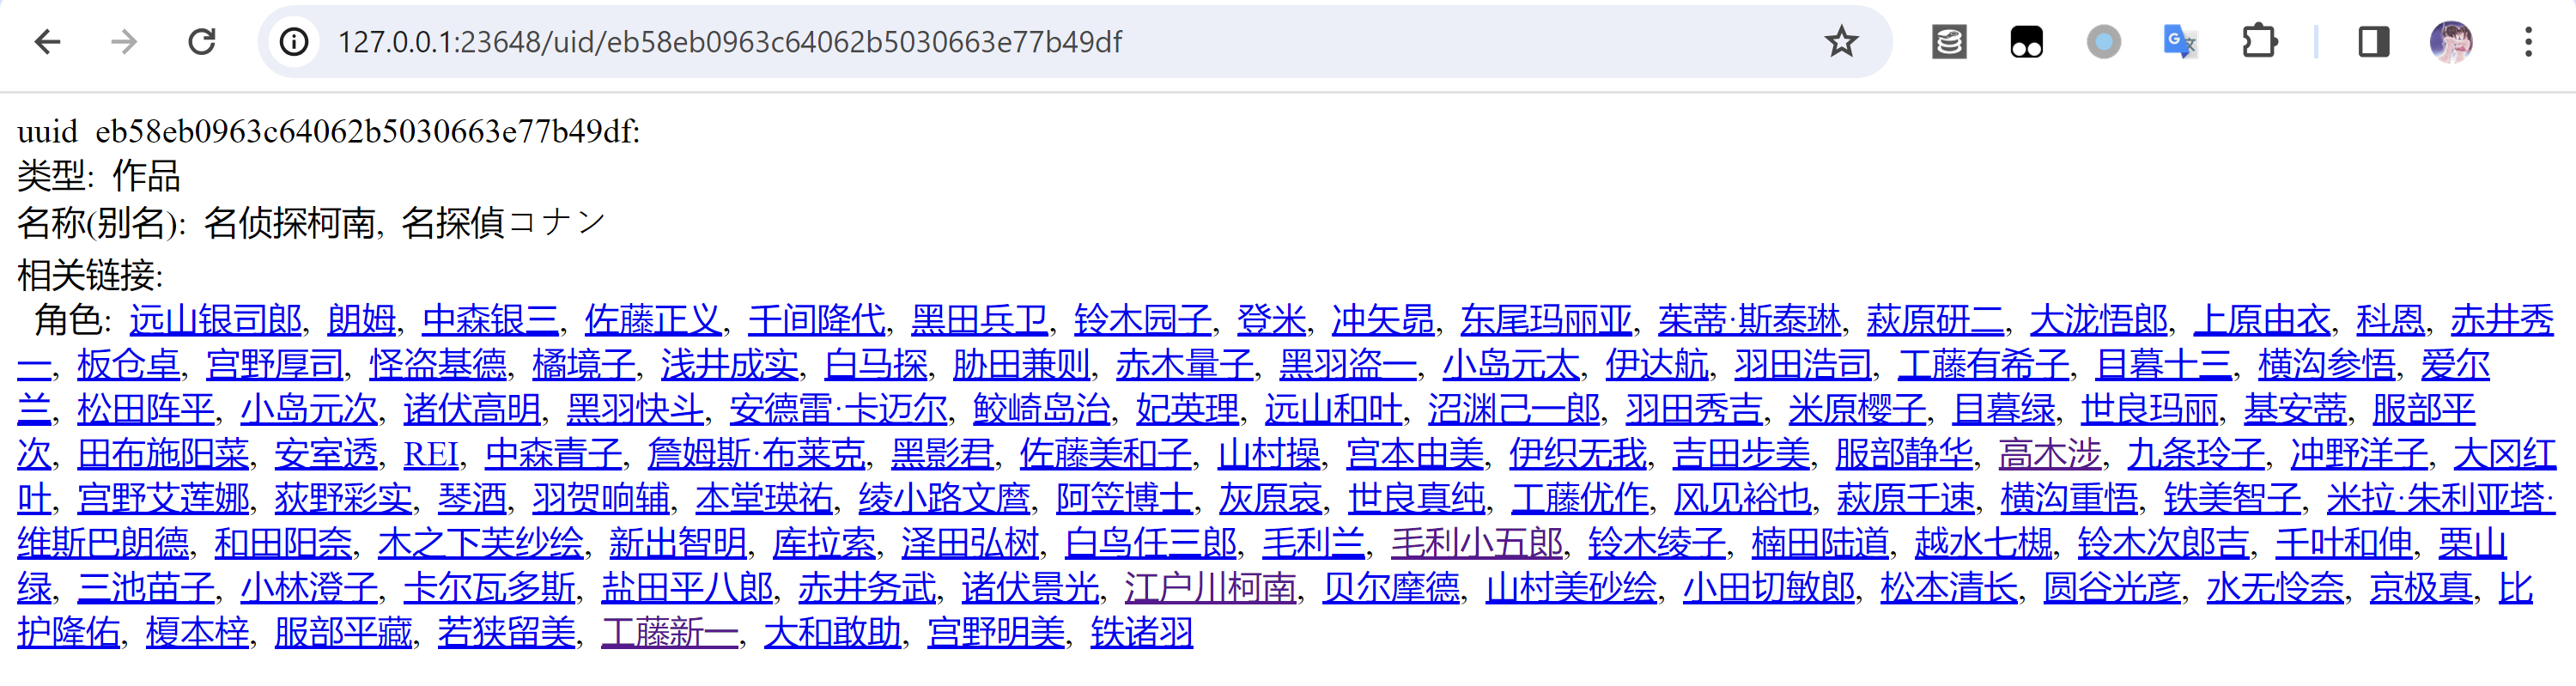
\includegraphics[height=.5\textheight]{pic/13.png}
    \end{figure}
\end{frame}

\section{QA}

\begin{frame}
    \begin{center}
        {\Huge\calligra Thanks!}
    \end{center}
\end{frame}

\end{document}
